\documentclass[letterpaper,11pt]{article}
\oddsidemargin -1.0cm \textwidth 17.5cm

\usepackage[utf8]{inputenc}
\usepackage[activeacute,spanish]{babel}
\usepackage{amsfonts,setspace}
\usepackage{amsmath}
\usepackage{amssymb, amsmath, amsthm}
\usepackage{comment}
\usepackage{amssymb}
\usepackage{dsfont}
\usepackage{anysize}
\usepackage{multicol}
\usepackage{enumerate}
\usepackage{graphicx}
\usepackage[left=1.5cm,top=2cm,right=1.5cm, bottom=1.7cm]{geometry}
\setlength\headheight{1.5em} 
\usepackage{fancyhdr}
\usepackage{multicol}
\usepackage{hyperref}
\usepackage{wrapfig}
\pagestyle{fancy}
\fancyhf{}
\renewcommand{\labelenumi}{\normalsize\bfseries P\arabic{enumi}.}
\renewcommand{\labelenumii}{\normalsize\bfseries (\alph{enumii})}
\renewcommand{\labelenumiii}{\normalsize\bfseries \roman{enumiii})}

\begin{document}

\fancyhead[L]{\itshape{Facultad de Ciencias F\'isicas y Matem\'aticas}}
\fancyhead[R]{\itshape{Universidad de Chile}}

\begin{minipage}{11.5cm}
    \begin{flushleft}
        \hspace*{-0.6cm}\textbf{FI1000-5 Introducción a la Física Clásica}\\
        \hspace*{-0.6cm}\textbf{Profesora:} Paulina Lira\\
        \hspace*{-0.6cm}\textbf{Auxiliares:} Alejandro Silva, Felipe Kaschel, Juan Cristobal Castro\\
    \end{flushleft}
\end{minipage}

\begin{picture}(2,3)
    \put(405,-5){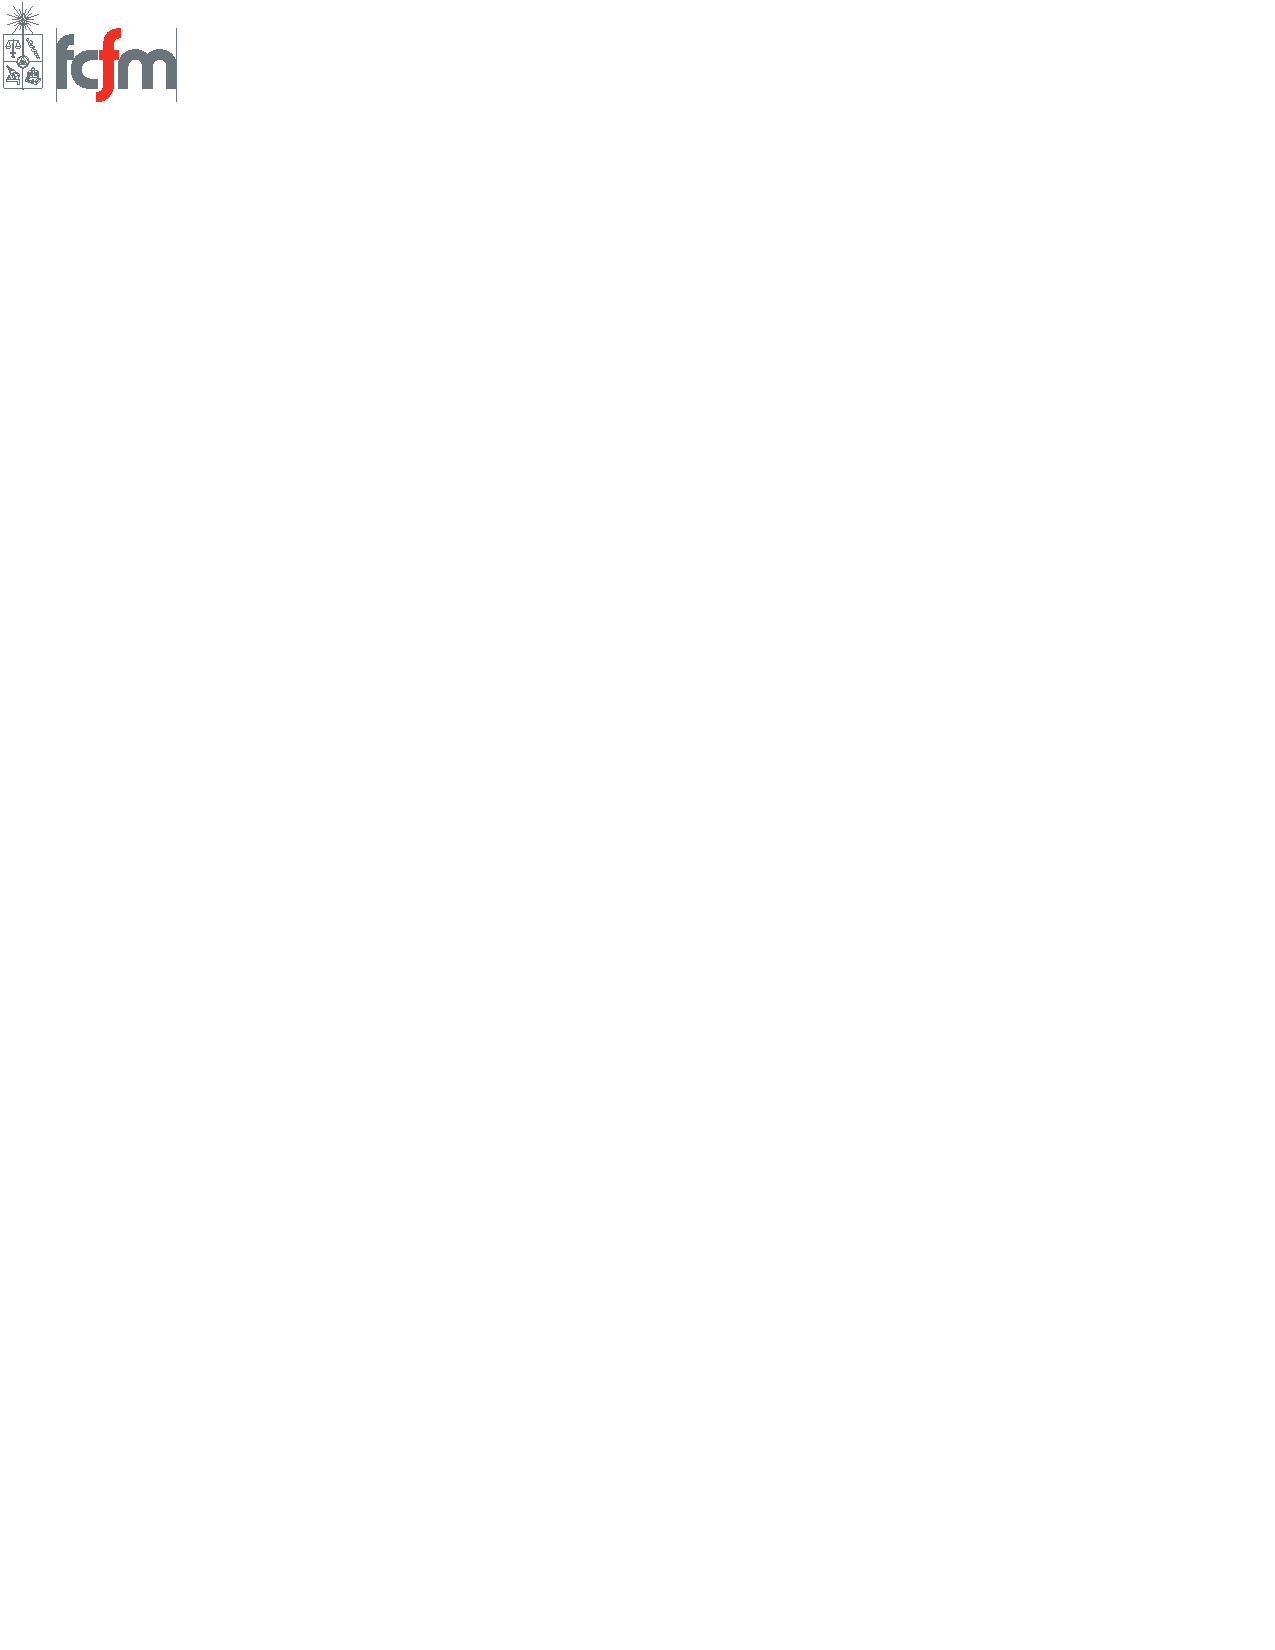
\includegraphics[scale=1.25]{2020-1/Imágenes/logo/fcfm2.pdf}}
\end{picture}

\begin{center}
	\LARGE \bf Auxiliar \#14: Estática de sólidos rígidos   \\
\end{center}

\vspace{-1cm}
\begin{enumerate}\setlength{\itemsep}{0.4cm}

\rfoot[]{pág. \thepage}

\item[]

\item Tenemos la configuración mostrada en la figura adjunta, en donde se conocen los valores de la masa $m_1$ y las distancias $x_1$ y $x_2$. Usted sabe que el balancín (sólido rígido) está en equilibrio estático, entonces se le pide lo siguiente.


a) calcule el valor de $m_2$ y $F$.

b) Demuestre que todo el sistema está en equilibrio, para esto tome otro punto de referencia y resuelva el problema mostrando que se obtienen los mismos resultados.
\\

\begin{figure}[h!]
        \centering
        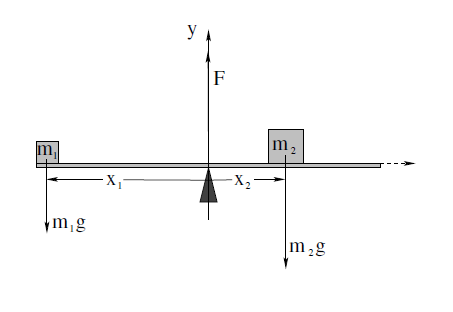
\includegraphics[scale=0.65]{2020-1/Imágenes/aux14/p1a14.png}
    \end{figure}


\item Una nueva empresa dedicada a entregar servicios de pintura de casas, decide poner publicidad en muchos puntos de la ciudad. Esta publicidad consta de un cartel sujeto desde la mitad de un soporte horizontal de largo $L$ no conocido. A su vez, este soporte descarga sobre un poste vertical por la izquierda que funciona de pivot, y también es sujetado por la derecha por un cable tensado que forma un ángulo $\theta$ con la horizontal.

Con la finalidad de comprar los materiales adecuados para las cargas solicitantes, la empresa le pide a usted que calcule las fuerzas $F_x$ y $F_y$ generadas en el punto pivot, además de la tensión $T$ del cable. Los únicos datos conocidos son  $\theta$ y $m$.
    
   \begin{figure}[h!]
        \centering
        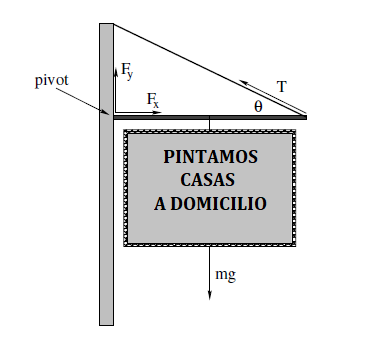
\includegraphics[scale=0.65
        ]{2020-1/Imágenes/aux14/p2a14}
    \end{figure} 
    
\newpage
    
\item  Una persona de masa $m$ se sube a una escalera de longitud $L$ y masa $M$, que está apoyada en una pared sin roce y un suelo rugoso. La escalera forma un ángulo $\alpha$ con la horizontal. El coeficiente de roce estático del suelo con la escalera está dado por $\mu$. ¿Hasta que altura con respecto al suelo puede subir la persona antes de que la escalera se caiga?\\

        

\end{enumerate}
\end{document}